\section{System perspective} \label{sp}
\subsection{Design and architecture} %% phbl 
The MiniTwit project is built using a single cloud-based  Virtual machine (\texttt{droplet}) with 1 CPU, 2 GB RAM, and 70 GB Storage, running 9 Docker containers in a Docker swarm setup. Three of these containers contain the MiniTwit replicas, written in Go with the \texttt{Gin} framework for web development. The decision to use Go was based on a desire to learn Go, but more importantly, due to the low memory usage and high efficiency of both Go and Gin, when compared to similar web frameworks and languages, such as C\# ASP.NET and Python using Flask \parencite{benchmark}. The MiniTwit application utilizes a cloud-based managed PostgreSQL database, since it allows the database to be retained even if the droplet is replaced. Additionally, to retain data and configuration files independently of droplets, an externally mounted volume with 20 GB of storage is required. Figure \ref{fig:Deployment} depicts the complete setup of deployed services

\begin{landscape}
\begin{figure}[H]
    \centering
    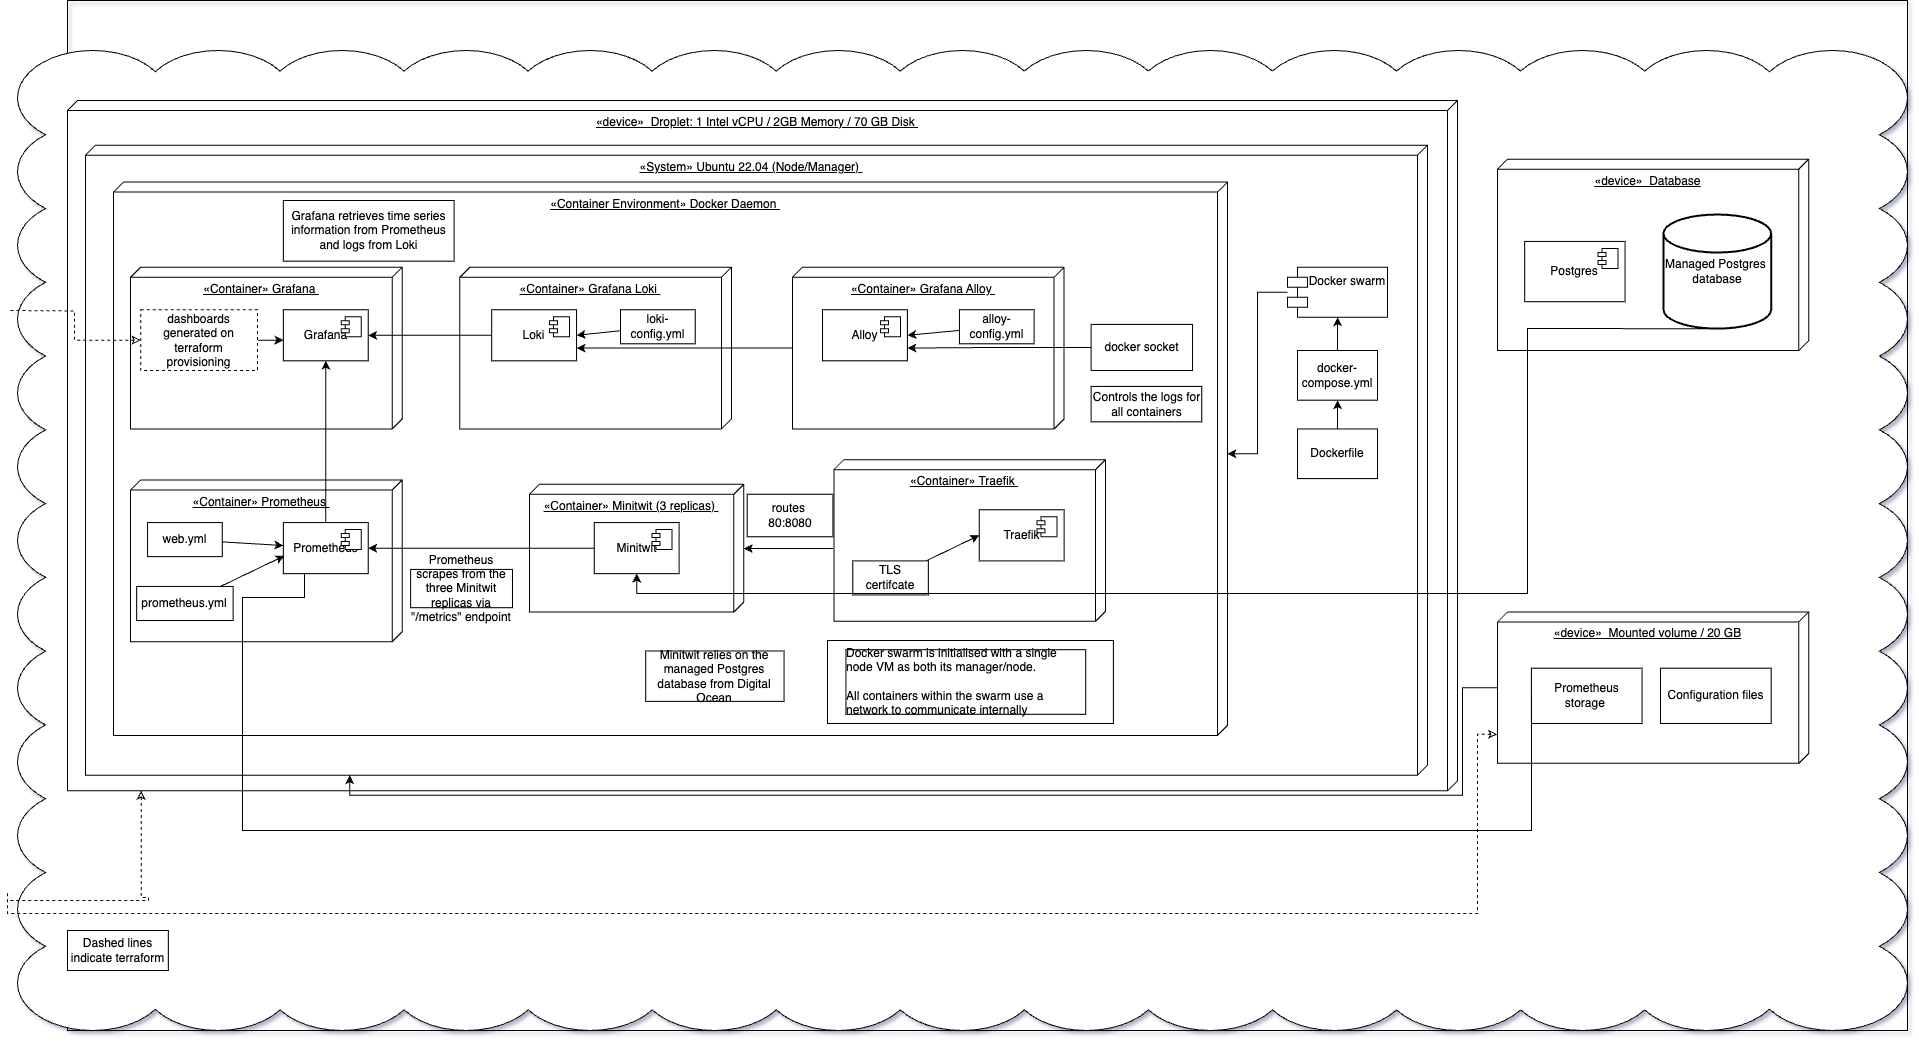
\includegraphics[width=1\linewidth]{pictures/UML.drawio (5).png}
    \caption{Deployment Diagram over MiniTwit project. On the right-hand side, there are some dashed lines, which indicate provisioning from Terraform, which is used for dashboard visualisations, and setting up a droplet, a database, and a mount.}
    \label{fig:Deployment}
\end{figure}
\end{landscape}


\subsection{Technology Stack and Motivations}

When making choices for the MiniTwit technology stack, we emphasised tools that allow for automation, declarative configuration, and scalability.

\begin{itemize}
    \item \textbf{GitHub with GitHub Actions, Projects, and Packages}: Serves as our central hub for version control, CI/CD pipelines, project management, and artifact repository. We chose GitHub because of its seamless integration with container registries, generous CI/CD minutes for public repositories, and robust ecosystem support. The integrated issue tracking and project boards eliminate the need for separate project management tools.

    \item \textbf{Terraform}: Manages infrastructure as code across multiple cloud providers. We selected Terraform because of its cloud-agnostic nature, allowing us to use the same tool for both deploying the infrastructure on DigitalOcean and the Grafana configuration. Its declarative syntax and state management prevent configuration drift that often occurs with imperative deployment scripts.

    \item \textbf{Docker}: Provides containerization for consistent deployment environments. Docker, together with Docker stack and Docker swarm, allowed us to express all of our services in a single file and manage all the communication and integration between them. It ensures our application runs identically across development, testing, and production.

    \item \textbf{DigitalOcean Spaces}: Handles log storage and terraform remote state. This solution was selected because it provides object storage compatible with S3 and also integrates seamlessly with our Alloy log service.

    \item \textbf{PostgreSQL}: Serves as our primary database. We chose PostgreSQL because it's a time-tested technology, open-source and provides great performance. PostgreSQL is also supported by DigitalOcean managed database service which decreased our operational burden.

    \item \textbf{Traefik}: Acts as our reverse proxy and SSL termination endpoint. Traefik was preferred over Nginx because of its automatic service discovery in Docker Swarm environments, through labels and a rich set of features. It also has built-in Let's Encrypt integration, which eliminates the need for manual certificate management.

    \item \textbf{Grafana}: Provides comprehensive visualization and alerting for system metrics. Grafana's extensive plugin ecosystem and multi-data source support allowed us to integrate all of our observability tools into one place.

    \item \textbf{Alloy}: Collects and forwards logs. Alloy was chosen because it is part of the Grafana ecosystem, maintained by the same organization and allows building complex log forwarding pipelines using a simple declarative syntax.

    \item \textbf{Loki}: Aggregates and stores application logs, and similarly to Allow, is part of the Grafana ecosystem, thus offering an effortless integration with Grafana. It was chosen for its simple setup and support for various external storage, including S3.

    \item \textbf{Prometheus}: Handles metrics collection. Prometheus is the industry standard for container-based monitoring, offering a powerful query language (PromQL) and a pull-based collection model that reduces operational complexity.

    \item \textbf{Golang}: Powers our backend application with excellent performance characteristics. Go was selected for its superior concurrency support, fast compilation times, and single binary deployment model. The single binary allowed us to build Docker images from scratch, achieving very small images and fast deployments.

    \item \textbf{Playwright}: Provides end-to-end testing capabilities. Playwright offers more reliable testing than Selenium-based solutions with built-in wait strategies and cross-browser support. We used TypeScript for defining the test suites and consider the developer experience offered by Playwright superior to Selenium.

    \item \textbf{Ansible}: Manages server configuration and application deployment. Ansible provides clear, version-controlled infrastructure configuration. Initially, we were using startup scripts for setting up the VM environment, but switched over to Ansible to be able to apply changes to the VM without having to re-create it. 

\end{itemize}
\subsection{Important interactions} % micje
%% A description of how interactions are made, and processed in the system. This should include an UML Sequence diagram, showing the aforementioned flow. 

%% This needs to be done both on an API level and a GUI-based level?

%% See component & connector viewpoint: https://github.com/itu-devops/lecture_notes/blob/master/sessions/session_13/Slides.md

Whenever a user opens or tries to interact with the web-application in any way, the control flow follows figure \ref{fig:user-seq}. This applies both to actual users and API requests that are made against the application. There is, however, a small change if it is an API request; instead of looking for the individual user, it instead tries to validate the API-key.

\begin{figure}[h!]
  \centering
  \includesvg[width=\textwidth]{pictures/User seq dia.svg}
  \caption{User sequence diagram}
  \label{fig:user-seq}
\end{figure}


\subsection{Current state} %% msro
%% A overview description of our results from the CI chain - testing,  Codeclimate and sonarqube. Everything is passing! 
%% Be sure to include metrics. 
We used several static analysis tools and tests to keep the
code in good shape. The current, most recent implementation
is working correctly and passing all tests, shown in figure \ref{fig:test-workflow}.

Below is an overview of two static code analysis tools applied to the current implementation:
\begin{itemize}
    \item SonarQube: 3.3k lines of code, 0 security issues (grade A), 5 reliability issues
    (grade C), 17 maintainability issues (grade A), 2.3\% code duplication
    (Below the suggested 3\% threshold), 237 cyclomatic complexity.
    \item CodeClimate: maintainability grade A, 5 code smells, 2 duplications,
    0 other issues.
\end{itemize}
